\begin{frame}
\frametitle{Densidad de estados}

\begin{itemize}
	\item{item 1} 
	\item{item 2}
\end{itemize}

\begin{figure}[h!]
\centering
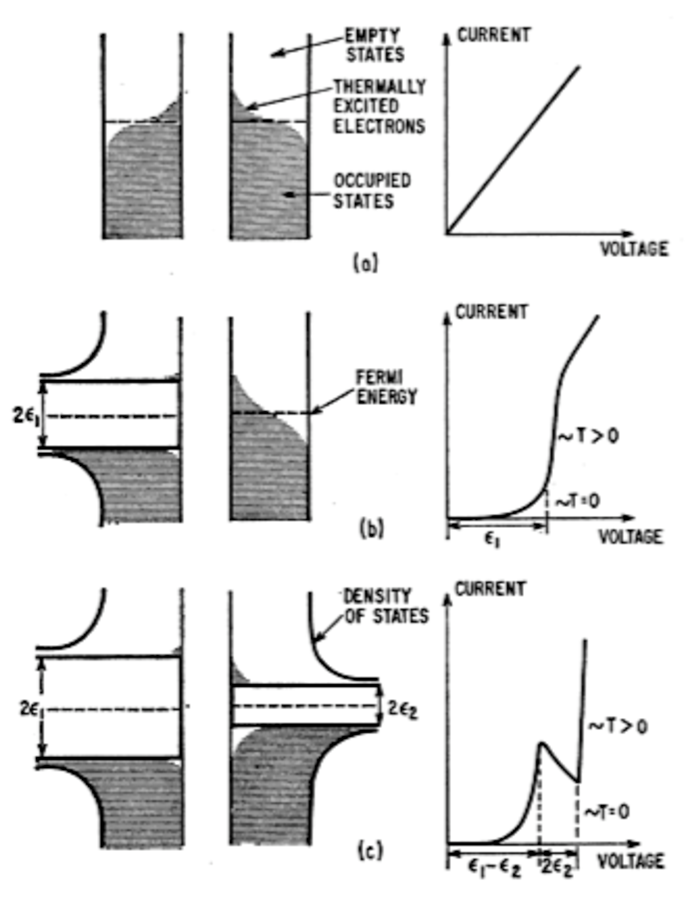
\includegraphics[width=0.45\textwidth]{fermi_levels}
\caption{\small Densidad de estados para los 3 casos
\label{fermi_levels}}
\end{figure}


\begin{center}
\textit{Uni\'on t\'unel...}
\end{center}

\end{frame}